\subsection*{Resultater}
Resultater har tre boundarys, hvor til der er opstillet en controlklasse. Boundarys og tilhørende controller fremgår af \autoref{fig:MVCresultater}. 

\begin{figure} [H]
\centering
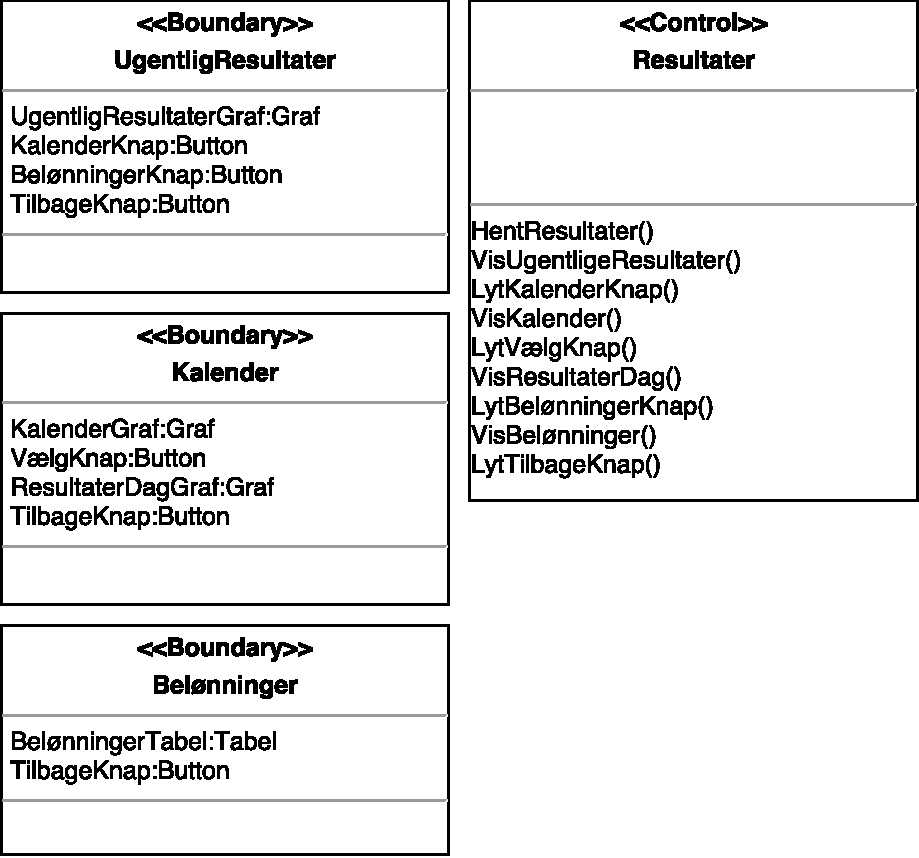
\includegraphics[width=0.8\textwidth]{figures/MVC/MVCResultater}
\caption{Designklasser for resultater. Til venstre ses de tre boundarys, UgentligResultater, Kalender og Belønninger. Til højre fremgår den tilhørende controller.}
\label{fig:MVCresultater}
\end{figure}

\noindent
I grænsefladerne er der grafer, tabeller og knapper. Disse er af typen Graf, Tabel og Button.  \fxnote{OBS!! Dette er stadig lidt uklart}. 
Controlleren for \textit{Resultater} indeholder Hent, Vis og Lyt metoder. 

I sammenspil med designklasserne for resultater er der udarbejdet et sekvensdiagram, hvilket fremgår af \autoref{fig:SEKResultater}

\begin{figure} [H]
\centering
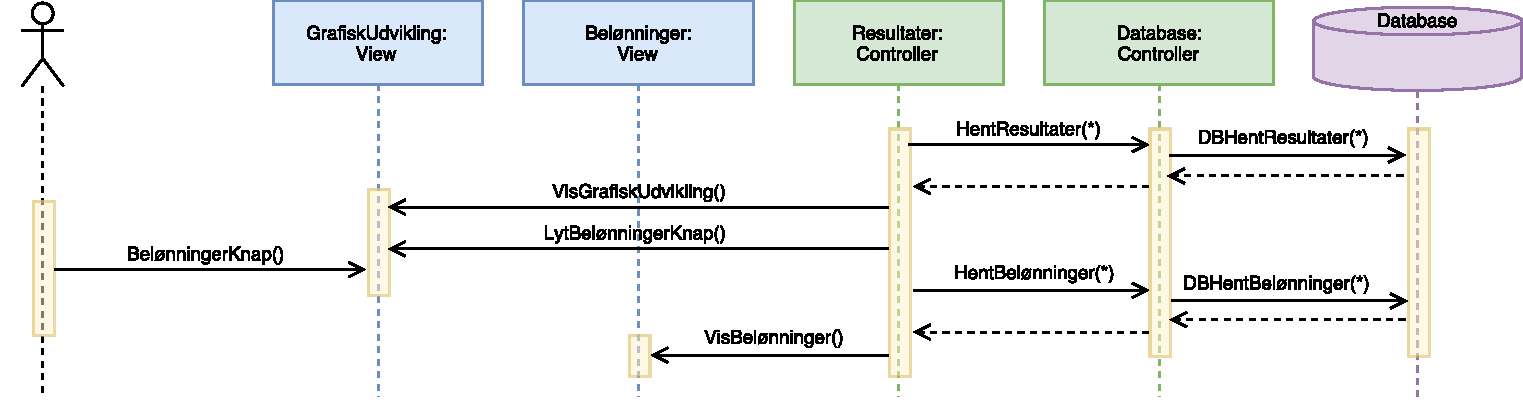
\includegraphics[width=1.55\textwidth, angle=90]{figures/Sek/SEKResultater}
\caption{Sekvensdiagram for Resultater.}
\label{fig:SEKResultater}
\end{figure} 

\noindent 
Når brugeren er tilgået resultater henter controlleren, \textit{KonditionResultater} resultater fra modellen \textit{KonditionResultater}.  Hvis brugeren endnu ikke har nogle resultater, vil disse ikke hentes, hvorved disse ikke vil vises i grænsefladerne. 

Grænsefladen \textit{UgentligResultater} viser ugentlige resultater i en graf.  Brugeren har mulighed for at trykke KalenderKnap eller BeløningerKnap. Trykker brugeren på KalenderKnap, vises grænsefladen for \textit{Kalender}, hvor brugeren har mulighed for at vælge en dag. Vælges dette, vises resultater i en graf for den valgte dag. Vælger brugeren at trykke på BelønningerKnap, viser grænsefladen \textit{Belønninger} en tabel med belønninger. Trykker brugeren ikke på en af knapperne, forbliver brugeren på grænsefladen for \textit{UgentligeResultater}

%Der er til \textit{ResultaterGrænseflade} opstillet en \textit{ResultatController}, der har til formål at hente nye resultater fra dagens træning i træningscontrolleren, når resultater tilgås via hovedmenugrænsefladen. Herefter vises en oversigtsgraf over udført træning. Træningscontrolleren fremgår af \autoref{fig:MVCTraening}.
%Controlleren lytter på om brugeren trykker på de angivne knapper i grænsefladen for resultater og viser valgt handling, hvis dette er tilfældet. 
